\documentclass[conference]{IEEEtran}
\IEEEoverridecommandlockouts
\usepackage[T1]{fontenc}
\usepackage[utf8]{inputenc}
\usepackage{amsmath,amssymb,amsfonts}
\usepackage{booktabs,tabularx,array,multirow}
\usepackage{graphicx}
\usepackage{tikz}
\usetikzlibrary{arrows.meta,positioning,fit,calc}
\usepackage[backend=biber,style=ieee,sorting=none]{biblatex}
\addbibresource{references.bib}
\usepackage{url}
\usepackage{balance}
\usepackage{microtype}
\usepackage{enumitem}
\setlist[itemize]{leftmargin=*,nosep,topsep=2pt}
\newcommand{\zktaf}{\textsc{ZK-TAF}}
\newcommand{\Com}{\mathsf{Com}}
\newcommand{\Hh}{\mathsf{H}}
\newcommand{\Verify}{\mathsf{Verify}}
\newcommand{\Prove}{\mathsf{Prove}}
\newcommand{\Auth}{\mathsf{Auth}}
\newcommand{\Accept}{\mathsf{Accept}}
\newcommand{\ttsmall}[1]{{\footnotesize\texttt{#1}}}
\title{ZK-TAF: Proof-Carrying x402 Payments for Policy-Gated Agentic Blockchain Finance}
\author{\IEEEauthorblockN{Anonymous Authors}\IEEEauthorblockA{Affiliations omitted for double-blind review}}
\begin{document}
\maketitle
\begin{abstract}
Autonomous AI agents can request priced services, invoke wallets, and submit blockchain payments, but a valid payment signature alone does not establish delegated authority, approved policy use, acceptable data freshness, or a faithful relationship between the approved action and the settled payment. Existing zero-knowledge machine learning (ZKML) systems establish selected computational claims, while HTTP-based x402 simplifies payment negotiation; neither mechanism, by itself, binds private financial controls to settlement. We develop \zktaf, a proposed proof-carrying payment design that gates a bounded on-chain financial action on a zero-knowledge relation over six properties: delegated authority, model/policy identity, oracle provenance and freshness, committed state continuity, deterministic risk controls, and exact payment binding. We distinguish model registry membership from evidence of actual model execution, specify attestation alternatives, and define an x402 v2 adapter with atomic settlement gating and replay protection. We present a formal security argument under stated trust assumptions, an adversarial test matrix, and a reproducible benchmark protocol against ungated, policy-only, and x402-only baselines. A reproducible local feasibility pilot evaluates payment-gate logic and a credential-bound Schnorr proof against four non-identical baselines. Across 100 clean and 180 encoded-attack trials per configuration, the pilot gate rejects all encoded attacks with no clean-request failures; an ablation without ZK attains the same rejection rate. These results are neither a six-property SNARK implementation nor evidence of live x402/EVM finality. The paper makes the trust assumptions and remaining verification gaps explicit.
\end{abstract}
\begin{IEEEkeywords}
agentic AI, blockchain, zero-knowledge proofs, x402, payment authorization, auditability, decentralized finance
\end{IEEEkeywords}

\section{Introduction}
Large-language-model (LLM) agents are moving from advice to financially consequential tool use, including market-data access, transaction construction, and payment for external services. A blockchain signature authenticates a signer but not the private decision process that led to its authorization. Conversely, making credentials, portfolio positions, model configuration, and raw observations public creates avoidable privacy and commercial exposure. An automated treasury agent may be legitimately delegated to purchase an API result for a fixed amount but should not be permitted to redirect the payment, exceed its cumulative budget, act on stale quotes, or reuse an old authorization.

The x402 protocol uses an HTTP \texttt{402 Payment Required} challenge, client-supplied signed payment authorization, and optional facilitator verification and settlement \cite{x402spec,solanax402}. It is a useful transport and payment-negotiation interface, \emph{not} a cryptographic statement about whether an AI agent followed a private mandate or policy. A server may rely on an external facilitator; the facilitator's signature checks also do not establish internal agent authorization. Independent zero-knowledge (ZK) systems enable verification of bounded statements about hidden inputs \cite{goldwasser1989,groth2016,plonk2019}, but model inference proofs, registry checks, and payment signatures are insufficient when enforced independently.

Our research question is: \emph{How can an agent's payment capability be conditioned on an auditable, privacy-preserving proof of its settlement-critical controls without presuming that cryptographic verification establishes model honesty or economic correctness?}

We contribute: (i) an explicit \emph{proof-before-privilege} payment interface that binds six assurance properties in a single state-transition statement; (ii) an x402 v2 integration design, with an enforceable on-chain gate rather than a purely advisory HTTP check; (iii) a tiered account of model provenance versus model execution, including its trust boundaries; and (iv) a falsifiable security and systems evaluation protocol covering transaction mutation, replay, oracle failures, liquidity shocks, and delayed or uncertain settlement. The novelty is \emph{system composition and its settlement boundary}, not a new proving algorithm. The present draft narrows the unit of analysis to a proof-carrying payment and includes a limited, reproducible local pilot; comprehensive zero-knowledge policy proving and live settlement measurements remain future work.

\section{Background and Research Gap}
\subsection{Independent proof and payment mechanisms}
Succinct arguments can verify arithmetic relations over private witnesses \cite{groth2016,plonk2019}; folding schemes such as Nova offer a path toward incremental verification \cite{nova2022}. ZKML research, including zkCNN, ZKML, and zkLLM, illustrates the costs and possibilities of proving selected ML computations \cite{zkcnn2021,zkml2024,zkllm2024}. None automatically authenticates a delegated financial mandate, an external oracle's economic truth, or the exact payment later sent by a wallet. Recent agent security benchmarks expose tool manipulation and prompt injection, underscoring the need for independent action controls \cite{toolemu2024,agentdojo2024}.

Oracle systems improve provenance and robustness but may still return economically misleading values \cite{acon22023}; privacy-preserving compliance and blockchain-enabled explainable federated credit scoring address complementary evidence problems rather than exact action gating \cite{buterin2024,jovanovic2024}. Existing payment protocols address transport, authorization, and settlement. The proposed missing unit is an \emph{atomic proof-carrying financial state transition} where approval, policy, data, state, and payment are bound together before value leaves an agent-controlled account.

\begin{table}[t]
\caption{What the proposed settlement gate adds (scope comparison, not measured superiority).}
\label{tab:gap}
\centering\footnotesize
\setlength{\tabcolsep}{3pt}
\begin{tabularx}{\columnwidth}{@{}lXXX@{}}
\toprule
Mechanism & Private controls & Payment semantics & Atomic gate \\
\midrule
ZKML proof & Selected ML relation & Not intrinsic & No \\
x402 v2 & No agent policy proof & Negotiation and signed payment & Not by itself \\
Policy-only wallet & Local deterministic predicates & Programmable payment & Trusts local enforcement \\
\zktaf{} (proposed) & Six-part ZK relation & Exact challenge/payment binding & Yes, if adapter enforces it \\
\bottomrule
\end{tabularx}
\end{table}

\section{System and Threat Model}
\subsection{Parties and confidential inputs}
A principal grants a restricted mandate to an agent runtime. A policy kernel evaluates hard financial limits independently of the agent's natural-language reasoning. A model registry, policy registry, delegation registry, oracle-root registry, and verifier-key registry publish authenticated version identifiers. The prover has private credentials, policy thresholds, portfolio state, authenticated observations, and evidence about the proposed action. A smart account or settlement adapter mediates fund release; an x402 resource server offers a priced service and may use a facilitator. A protected audit store retains selected encrypted evidence, while a receipt anchors its version commitments.

Let \(s_t\) denote private committed state, \(d_t\) a delegated mandate, \(m_t\) a model/configuration descriptor, \(p_t\) a policy, \(o_t\) signed oracle evidence, \(q_t\) x402 challenge/requirements, and \(a_t\) the canonical proposed payment. We assume collision-resistant hashing, hiding/binding commitments, and a complete/sound ZK proof system; key and registry trust must be operationally governed rather than inferred from cryptography. A compromised oracle signer can certify a false value, and a compromised attestation authority can falsely attest execution. The proposed control blocks unauthorised \emph{encoded} financial effects, not every harmful semantic decision an agent might make.

\subsection{Trust boundaries}
Table~\ref{tab:trust} distinguishes attack resistance from retained trust. We assume the settlement contract is correctly deployed, remains the exclusive route for spending designated funds, and checks current registry state atomically. A conventional x402 payment signature that can independently settle via a direct token transfer \emph{bypasses this guarantee}; the design requires a compatible gated scheme, escrow, or smart-account policy, and existing x402 facilitators cannot be assumed to support that scheme without an explicit adapter.

\begin{table}[t]
\caption{Dependencies, failures, and consequences.}
\label{tab:trust}
\centering\footnotesize
\setlength{\tabcolsep}{3pt}
\begin{tabularx}{\columnwidth}{@{}p{.22\columnwidth}XX@{}}
\toprule
Dependency & Required assumption & Residual risk / containment \\
\midrule
Registry owner & Controlled updates and rotation & Malicious approval; multisig, delay, revoke \\
Oracle committee & Signed, recent root & Fresh but false price; diversity and bounds \\
Model attester & Verified measurement and key binding & Compromised TEE / key; revocation, T2 proof \\
Facilitator & Network/capability correctly reported & Misreported or pending settlement; on-chain reconciliation \\
RPC/chain & Correct finality and chain identity & Reorg/latency; confirmations and expiry \\
Gate/keys & Exclusivity of spend path & Alternate transfer path defeats assurance \\
\bottomrule
\end{tabularx}
\end{table}

\section{ZK-TAF Architecture and Formal Relation}
\subsection{Proof-before-privilege}
Figure~\ref{fig:architecture} shows the crucial separation between off-chain reasoning and on-chain authority. The agent may produce an arbitrary private tool trace, but the gate decides only whether a fixed action satisfies a circuit-friendly relation. Sensitive identity attributes, private thresholds, oracle observations, and portfolio details remain witnesses; version commitments, a bounded expiry, and an action digest are public. The resulting receipt is evidence of predicates checked \emph{at a particular epoch}, not a public explanation of the agent's reasoning.

\begin{figure*}[t]
\centering
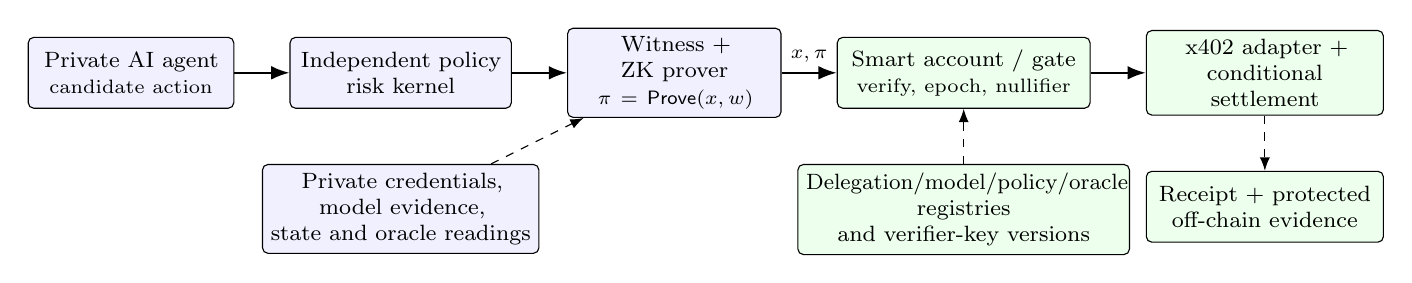
\begin{tikzpicture}[>=Latex, node distance=7mm and 7mm, every node/.style={font=\footnotesize}, n/.style={draw,rounded corners=2pt,align=center,minimum height=9mm,inner sep=3pt}, priv/.style={n,fill=blue!6}, pub/.style={n,fill=green!7}]
\node[priv,text width=24mm] (agent) {Private AI agent\\\scriptsize candidate action};
\node[priv,text width=26mm,right=of agent] (kernel) {Independent policy\\risk kernel};
\node[priv,text width=25mm,right=of kernel] (prover) {Witness + ZK prover\\\scriptsize $\pi=\Prove(x,w)$};
\node[pub,text width=30mm,right=of prover] (gate) {Smart account / gate\\\scriptsize verify, epoch, nullifier};
\node[pub,text width=28mm,right=of gate] (settle) {x402 adapter +\\conditional settlement};
\draw[->,thick] (agent)--(kernel);
\draw[->,thick] (kernel)--(prover);
\draw[->,thick] (prover)-- node[above,midway] {\scriptsize $x,\pi$} (gate);
\draw[->,thick] (gate)--(settle);
\node[priv,below=7mm of kernel,text width=33mm] (inputs) {Private credentials, model evidence,\\state and oracle readings};
\node[pub,below=7mm of gate,text width=40mm] (registry) {Delegation/model/policy/oracle registries\\and verifier-key versions};
\node[pub,below=7mm of settle,text width=28mm] (receipt) {Receipt + protected\\off-chain evidence};
\draw[->,dashed] (inputs)--(prover);
\draw[->,dashed] (registry)--(gate);
\draw[->,dashed] (settle)--(receipt);
\end{tikzpicture}
\caption{Proposed proof-before-privilege architecture. Dashed dependencies provide authenticated private evidence, trusted public parameters, and audit anchoring; only the smart-account gate can release the governed funds.}
\label{fig:architecture}
\end{figure*}

Define an unambiguous, typed canonical encoding \(\mathsf{Enc}\) of fields rather than hashing arbitrary JSON. A payment descriptor is
\begin{equation}
\begin{aligned}
 a_t=(\,&\textsf{net},\textsf{scheme},\textsf{asset},\textsf{payTo},\textsf{amt},\\
      &\textsf{resource},\textsf{reqHash},\textsf{nonce},\textsf{deadline}\,).
\end{aligned}
 \label{eq:action}
\end{equation}
Network uses a canonical chain identifier; \(\textsf{reqHash}\) commits to the full selected x402 v2 requirements, including any extension data and its domain. The digest
\begin{equation}
 h_a=\Hh(\textsf{``ZKTAF-PAY-v1''}\parallel\mathsf{Enc}(a_t)\parallel\textsf{gateAddress})
 \label{eq:hash}
\end{equation}
prevents cross-domain reuse and post-proof modification. The public statement, with commitments hiding private identities and state, is
\begin{equation}
 x_t=(h_D,h_M,h_P,h_O,S_t,S_{t+1},h_a,e,\nu_t,T_t,v),
 \label{eq:public}
\end{equation}
where \(e\) is a registry/oracle epoch, \(\nu_t\) a unique nullifier, \(T_t\) a deadline, and \(v\) a circuit/verifier version. The witness \(w_t\) contains opening information for credentials, model/policy evidence, private state, oracle leaves and authenticated paths, risk data, and the proposed action. Model execution evidence is additional to \(h_M\), as discussed next.

The composite relation is
\begin{equation}
 R(x_t,w_t)=R_D\land R_M\land R_O\land R_S\land R_K\land R_A=1.
 \label{eq:relation}
\end{equation}
Here \(R_D\) proves valid delegation and scope; \(R_M\) binds approved model \emph{and} policy identities, with execution assurance level recorded separately; \(R_O\) proves oracle-signer membership, accepted epoch, and age bound; \(R_S\) proves \(S_{t+1}=\Com(F(s_t,a_t,o_t))\) with consistent openings; \(R_K\) proves budget, destination, slippage, and value/risk limits; and \(R_A\) proves \(h_a\) corresponds to the exact payment encoded in the verifier's transaction. Budget limits must use a committed cumulative counter and an atomic update: proving a per-payment threshold alone does not prevent concurrent overspending.

On chain, the designated contract authorizes settlement iff
\begin{multline}
\Accept=\Verify(vk_v,x_t,\pi_t)\wedge\mathsf{Current}(e,v)\\
\wedge\neg\mathsf{Used}(\nu_t)\wedge\mathsf{Now}\leq T_t
\wedge\mathsf{Digest}(a_t)=h_a\\
\wedge\mathsf{StateRoot}=S_t\wedge\mathsf{SpendPath}=\textsf{Gate}.
\label{eq:gate}
\end{multline}
Here, \(\mathsf{Digest}\) denotes the domain-separated construction in (\ref{eq:hash}). The gate consumes the nullifier, updates the state root and releases payment \emph{within the same atomic state transition}; any failed subcheck reverts. This is an architecture specification, not a verified Solidity implementation.

\subsection{Model identity is not execution evidence}
A model hash only proves that an approved descriptor was referenced; it does \emph{not} prove a model produced an output. We distinguish three assurance tiers: \textbf{T0}, registry-only identification (weakest); \textbf{T1}, remote execution attestation binding a measured runtime, model commitment, input/output digests, time window, and action nonce (trusts the attester, hardware, and runtime); and \textbf{T2}, verifiable computation proving a bounded model/inference or policy-relevant subcomputation (greater proving cost and coverage limits). A T1 signature may be verified inside the ZK relation using a supported signature circuit, or verified outside the circuit if its authenticated digest is unambiguously included in the gated statement. \emph{None} of T0--T2 proves good judgment, harmless prompts, or truthful external data. An experiment should report the chosen tier, attacker capability, and any gap between model output and finalized action.

\section{x402 v2 Settlement Adapter}
The HTTP v2 workflow negotiates offers through \texttt{PAYMENT-REQUIRED}, submits a signed payload via \texttt{PAYMENT-SIGNATURE}, and returns settlement information through \texttt{PAYMENT-RESPONSE} \cite{x402spec}. We propose a \zktaf{} adapter that reads the full payment requirement, freezes the canonical typed payment descriptor, and adds a proof-reference extension recognized by both the resource server and the facilitator or equivalent self-facilitated service. x402 itself neither requires nor universally understands such an extension.

The key deployment decision concerns \emph{fund control}. A regular directly settleable token authorization must not coexist with a policy-only off-chain proof check: another party might redeem it without invoking the gate. The proposed implementation therefore routes settlement through a constrained smart account or escrow holding the funds and accepts only proof-gated transactions. The resource server checks the settlement receipt and resource-specific binding before delivery; it must not infer success from a facilitator's mere preflight \texttt{/verify} response. A pending or indeterminate \texttt{/settle} result triggers on-chain reconciliation rather than a second transfer \cite{x402fac}.

\noindent\textbf{Protocol (proposed):}
\begin{enumerate}[leftmargin=*,nosep]
\item Fetch x402 \texttt{402} challenge; select supported scheme, network, asset, and offer; reject if the chosen facilitator/gate lacks capability.
\item Validate delegation and registry epochs; obtain authenticated oracle evidence and current state root.
\item Produce candidate payment, independently evaluate deterministic policy, and fix the typed encoding and request hash.
\item Produce model-execution evidence at the declared tier, create \(x_t\), and generate \(\pi_t\) only after action bytes are fixed.
\item Submit action, proof, and replay nullifier to the exclusive settlement gate; recheck the current epoch and state atomically.
\item On success, record the final chain receipt, return an x402-compatible settlement response, and release the resource; on pending confirmation, reconcile without double charge.
\end{enumerate}

\begin{table}[t]
\caption{Security experiments and falsifiable acceptance checks (not observed results).}
\label{tab:attacks}
\centering\footnotesize
\setlength{\tabcolsep}{3pt}
\begin{tabularx}{\columnwidth}{@{}p{.24\columnwidth}XX@{}}
\toprule
Injected fault & Expected gate outcome & Required evidence \\
\midrule
Amount/payee/asset mutation & Reject & Frozen bytes and revert \\
Nonce replay / other chain & Reject & Used-nullifier/domain log \\
Expired delegation/policy & Reject & Version/epoch rollback trace \\
Concurrent budget payments & At most permitted total & Atomic state-root history \\
Stale oracle root / age & Reject & Signed epoch/age traces \\
Fresh but false oracle price & May pass & False-data counterexample \\
Compromised attester (T1) & Outside guaranteed scope & Failure injection and trust boundary \\
Facilitator timeout / reorg & Pending/reconcile & No duplicate finalized debit \\
Liquidity/slippage shock & Reject if threshold encoded & Quote-to-finality delta \\
\bottomrule
\end{tabularx}
\end{table}

\section{Security Claims and Limitations}
\textbf{Claim 1 (exact-action integrity).} Under soundness, collision resistance, an exclusive gate, and atomic state updates, an accepted payment must match the action digest and satisfy every correctly implemented predicate in (\ref{eq:relation}). \emph{Argument:} otherwise either an invalid witness produced an accepted proof, a different encoded action matched the digest, or an alternative spend path bypassed the gate. This is a reduction-style design argument, not a machine-checked proof.

\textbf{Claim 2 (replay and budget).} Domain-separated nullifiers and serializable state-root checks reject repeated settlement and prevent concurrently accepted transactions from jointly exceeding \emph{encoded} aggregate limits, assuming the same account/gate and atomic execution. Cross-chain transfers require coordinated state or independent scoped budgets; an isolated chain cannot guarantee a global limit without cross-chain finality assumptions.

\textbf{Claim 3 (selective confidentiality).} Zero knowledge protects the witness relative to the public statement, not addresses, service endpoints, transaction timing, token amounts if they are public, event correlation, or inferences from economic effects. Stable identifiers and repeated receipt publication may defeat unlinkability; rotating nullifiers and limiting receipt fields reduce but do not remove exposure.

These claims fail if the circuit omits a required condition, registries are malicious, the attester lies, the oracle has validly signed false data, or signed payment rights bypass the gate. They do not certify legal compliance or economic optimality. To avoid an artificial ``fully trusted verifier'' assumption, the benchmark must publish contract code, circuit/VK hashes, registry governance, attestation tier, oracle-signature policy, and which components operators can replace unilaterally.

\section{Evaluation Protocol and Reproducibility}
\subsection{Prototype and comparative baselines}
The primary deployment target is an EVM-compatible testnet, using an x402 v2 \texttt{exact} payment for a priced data/API resource. A minimal reproducible prototype should include: a constrained payer smart account; a typed x402 payment adapter; delegation, model, policy, verifier-key, and oracle registries; a Groth16 or PLONK circuit for a bounded payment-risk relation; a prover service; an authenticated oracle-root publisher; a verifier/gate contract; and encrypted off-chain audit records. Publish compiler/tool versions, chain height, hardware, workloads, circuit constraint counts, and raw measurement scripts. A single synthetic workload is insufficient for external-validity claims; include trace-based financial activity or clearly labelled realistic workloads where licensing/privacy permit.

Compare four independent configurations on the same service, network, workload, and wallets: \textbf{A}: ungated agent; \textbf{B}: local deterministic policy check; \textbf{C}: conventional x402 authorization/settlement (payment integrity but no agent proof); and \textbf{D}: proposed \zktaf{} with gated settlement and a declared T0/T1/T2 model-assurance tier. An additional \textbf{D-noZK} ablation uses the same on-chain deterministic gate with public inputs to separate proof privacy/overhead from mere on-chain enforcement. Chainlink Proof of Reserve and other reserve-attestation systems may be compared for trust-model coverage, but must \emph{not} be described as direct transaction-gating performance baselines because they attest different properties.

\subsection{Measures and experimental design}
Test clean requests and injected attacks listed in Table~\ref{tab:attacks}. Repeat each configuration over controlled network conditions and multiple transaction sizes, then report median, p95, confidence intervals, and raw counts rather than only averages. Primary dependent variables are: proof generation/verification time, peak prover memory, proof size, on-chain gas and total fees, end-to-end HTTP request-to-finality latency, throughput, success and false-rejection rates, prohibited-action acceptance rate, duplicate-payment incidents, and audit reconstruction completeness. Compare \(T_0\), \(T_1\), and feasible bounded \(T_2\) to expose model-attestation costs.

Model liquidity shocks by changing quote-to-settlement price and available pool depth, including adverse movement across the slippage threshold. Simulate oracle silence, key compromise, outdated membership roots, registry revocation between proof and settlement, facilitator timeout after transaction broadcast, chain reorganisation, and simultaneous payment requests. For multi-chain experiments, report bridging assumptions and the time until cross-chain state consistency; do not assume instant atomicity. To measure privacy, examine both witness contents and linkability from on-chain/public HTTP metadata. Audit experiments should test whether a reviewer can reconstruct action/mandate/policy/oracle linkage from the receipt plus selectively revealed records without obtaining unneeded portfolio or prompt information.

\subsection{Local pilot implementation and observed results}
We implemented an \emph{off-chain, synthetic feasibility pilot} of the payment authorisation boundary in Python 3 using Ed25519 signatures and a Fiat--Shamir Schnorr proof over a 2048-bit MODP subgroup. The Schnorr statement proves \emph{knowledge of a credential secret bound to a canonical action digest}, not satisfaction of the six ZK-TAF properties in zero knowledge. Financial constraints, freshness, epoch, and replay are evaluated explicitly at the local gate. This surrogate is \textbf{D*}, not the proposed full on-chain D. \textbf{C*} simulates signed x402-like payments, not a live x402 server or facilitator. Configuration \textbf{E} is the same local deterministic gate as D* without the credential proof. The policy-only B checks at preflight rather than atomically at settlement.

For each configuration, we ran 100 clean requests, 20 repetitions of each of nine encoded attack categories, and 20 fresh-but-false-oracle cases (300 cases per configuration; 1,500 in total). The seeded scenarios cover amount/payee violations, stale feeds, post-check mutation, replay, revocation, wrong chain, adverse quote movement, and timeout/retry. Two retry scenarios attempt a second debit. All cases run in one local process without HTTP, real agents, a blockchain, or block confirmation. Table~\ref{tab:results} reports observed counts and host-dependent timing; raw logs and the script accompany the artifact.

\begin{table}[t]
\caption{\emph{Measured local pilot only}; not full ZK-TAF or on-chain x402 performance.}
\label{tab:results}
\centering\footnotesize
\setlength{\tabcolsep}{2.7pt}
\begin{tabular}{@{}lccccc@{}}
\toprule
Metric & A & B & C* & D* & E \\
\midrule
Clean accepted (\%) & 100 & 100 & 100 & 100 & 100 \\
Encoded attacks accepted (\%) & 100 & 66.7 & 55.6 & 0 & 0 \\
False fresh oracle accepted (\%) & 100 & 100 & 100 & 100 & 100 \\
Local request p95 (ms) & .001 & .002 & .294 & 88.11 & .016 \\
Credential prover p95 (ms) & -- & -- & -- & 33.02 & -- \\
Duplicate local debits (count) & 40 & 40 & 0 & 0 & 0 \\
End-to-end finality p95 (s) & NM & NM & NM & NM & NM \\
EVM gas per payment & NM & NM & NM & NM & NM \\
\bottomrule
\end{tabular}
\vspace{2pt}
\begin{minipage}{\columnwidth}\scriptsize
A: ungated; B: preflight-only policy; C*: x402-like signed action; D*: local gated Schnorr credential proof; E: gate without proof. Each column: 100 clean, 180 encoded attacks, 20 false-oracle trials. NM: no deployment/measurement; --: not applicable. Timings are Python host measurements, \emph{not} network/finality latency.\end{minipage}
\end{table}

All 180/180 encoded attacks are rejected by D* and E, compared with 0/180 rejected by A, 60/180 by B, and 80/180 by C*. The identical D*/E rejection rates establish that the local gate's checks, \emph{not the added proof}, account for those results. All five accept the 20/20 cases in which fresh, purportedly authenticated oracle values are economically false, confirming the stated external-truth limitation. The credential proof adds substantial Python-level overhead (D* request p95 88.11\,ms; standalone prover p95 33.02\,ms); these timings cannot be transferred to optimised Groth16/PLONK systems. No gas, blockchain finality, witness-privacy, throughput-under-load, or actual x402 interoperability claim follows from this pilot.

The \emph{future full-system acceptance objective} remains zero accepted mutation/replay cases under encoded predicates and exclusive gate assumptions. A conference-ready implementation must replace D* with an auditable six-property ZK circuit and EVM verifier, measure real gas and request-to-finality latency, and include replayable trace-based workloads. The pilot provides limited executable feasibility evidence, not validation of the proposed cryptographic architecture.

\section{Governance and Deployment Considerations}
Model approval, credential checks, and ZK receipts can support auditable evidence, but cannot resolve human oversight, legal qualification, or adequacy of policy. EU AI Act applicability depends on intended use and classification; GDPR may still apply to pseudonymous commitments if individuals can be linked \cite{aiact2024,gdpr2016}. A two-tier audit model publishes minimal commitments and retains encrypted detailed records with retention, access controls, and selective disclosure. Regulators still need external context, organizational records, and legal interpretation. For deployment, mandate revocation, signer compromise, incident recovery, verifier-key upgrade, model/version rollback, and emergency freezes require documented procedures, not just a circuit specification.

\section{Conclusion}
\zktaf{} specifies a proof-before-privilege boundary for agent-initiated blockchain payments, composing delegated authority, approved versions, oracle provenance/freshness, state continuity, deterministic financial limits, and exact payment binding. Its x402 v2 adapter makes payment negotiation interoperable while requiring a separately enforceable settlement gate; x402 by itself is not an assurance system. Model execution requires its own attestation or verifiable-computation evidence, not a registry hash alone. The reproducible local pilot confirms rejection of the encoded attacks by a deterministic gate and exposes oracle-truth and proving-overhead limitations; an ablation shows that the credential proof does not improve these local rejection outcomes. Full six-property private verification, x402 protocol compatibility, live EVM gas/finality, production deployability, and regulatory compliance remain unvalidated. The next step is to implement and evaluate the proposed proof circuit and exclusive on-chain gate.

\printbibliography
\end{document}